% Options for packages loaded elsewhere
\PassOptionsToPackage{unicode}{hyperref}
\PassOptionsToPackage{hyphens}{url}
%
\documentclass[
]{article}
\usepackage{lmodern}
\usepackage{amsmath}
\usepackage{ifxetex,ifluatex}
\ifnum 0\ifxetex 1\fi\ifluatex 1\fi=0 % if pdftex
  \usepackage[T1]{fontenc}
  \usepackage[utf8]{inputenc}
  \usepackage{textcomp} % provide euro and other symbols
  \usepackage{amssymb}
\else % if luatex or xetex
  \usepackage{unicode-math}
  \defaultfontfeatures{Scale=MatchLowercase}
  \defaultfontfeatures[\rmfamily]{Ligatures=TeX,Scale=1}
\fi
% Use upquote if available, for straight quotes in verbatim environments
\IfFileExists{upquote.sty}{\usepackage{upquote}}{}
\IfFileExists{microtype.sty}{% use microtype if available
  \usepackage[]{microtype}
  \UseMicrotypeSet[protrusion]{basicmath} % disable protrusion for tt fonts
}{}
\makeatletter
\@ifundefined{KOMAClassName}{% if non-KOMA class
  \IfFileExists{parskip.sty}{%
    \usepackage{parskip}
  }{% else
    \setlength{\parindent}{0pt}
    \setlength{\parskip}{6pt plus 2pt minus 1pt}}
}{% if KOMA class
  \KOMAoptions{parskip=half}}
\makeatother
\usepackage{xcolor}
\IfFileExists{xurl.sty}{\usepackage{xurl}}{} % add URL line breaks if available
\IfFileExists{bookmark.sty}{\usepackage{bookmark}}{\usepackage{hyperref}}
\hypersetup{
  pdftitle={Gestion de Portefeuille},
  pdfauthor={Patrick Hénaff},
  hidelinks,
  pdfcreator={LaTeX via pandoc}}
\urlstyle{same} % disable monospaced font for URLs
\usepackage[margin=1in]{geometry}
\usepackage{color}
\usepackage{fancyvrb}
\newcommand{\VerbBar}{|}
\newcommand{\VERB}{\Verb[commandchars=\\\{\}]}
\DefineVerbatimEnvironment{Highlighting}{Verbatim}{commandchars=\\\{\}}
% Add ',fontsize=\small' for more characters per line
\usepackage{framed}
\definecolor{shadecolor}{RGB}{248,248,248}
\newenvironment{Shaded}{\begin{snugshade}}{\end{snugshade}}
\newcommand{\AlertTok}[1]{\textcolor[rgb]{0.94,0.16,0.16}{#1}}
\newcommand{\AnnotationTok}[1]{\textcolor[rgb]{0.56,0.35,0.01}{\textbf{\textit{#1}}}}
\newcommand{\AttributeTok}[1]{\textcolor[rgb]{0.77,0.63,0.00}{#1}}
\newcommand{\BaseNTok}[1]{\textcolor[rgb]{0.00,0.00,0.81}{#1}}
\newcommand{\BuiltInTok}[1]{#1}
\newcommand{\CharTok}[1]{\textcolor[rgb]{0.31,0.60,0.02}{#1}}
\newcommand{\CommentTok}[1]{\textcolor[rgb]{0.56,0.35,0.01}{\textit{#1}}}
\newcommand{\CommentVarTok}[1]{\textcolor[rgb]{0.56,0.35,0.01}{\textbf{\textit{#1}}}}
\newcommand{\ConstantTok}[1]{\textcolor[rgb]{0.00,0.00,0.00}{#1}}
\newcommand{\ControlFlowTok}[1]{\textcolor[rgb]{0.13,0.29,0.53}{\textbf{#1}}}
\newcommand{\DataTypeTok}[1]{\textcolor[rgb]{0.13,0.29,0.53}{#1}}
\newcommand{\DecValTok}[1]{\textcolor[rgb]{0.00,0.00,0.81}{#1}}
\newcommand{\DocumentationTok}[1]{\textcolor[rgb]{0.56,0.35,0.01}{\textbf{\textit{#1}}}}
\newcommand{\ErrorTok}[1]{\textcolor[rgb]{0.64,0.00,0.00}{\textbf{#1}}}
\newcommand{\ExtensionTok}[1]{#1}
\newcommand{\FloatTok}[1]{\textcolor[rgb]{0.00,0.00,0.81}{#1}}
\newcommand{\FunctionTok}[1]{\textcolor[rgb]{0.00,0.00,0.00}{#1}}
\newcommand{\ImportTok}[1]{#1}
\newcommand{\InformationTok}[1]{\textcolor[rgb]{0.56,0.35,0.01}{\textbf{\textit{#1}}}}
\newcommand{\KeywordTok}[1]{\textcolor[rgb]{0.13,0.29,0.53}{\textbf{#1}}}
\newcommand{\NormalTok}[1]{#1}
\newcommand{\OperatorTok}[1]{\textcolor[rgb]{0.81,0.36,0.00}{\textbf{#1}}}
\newcommand{\OtherTok}[1]{\textcolor[rgb]{0.56,0.35,0.01}{#1}}
\newcommand{\PreprocessorTok}[1]{\textcolor[rgb]{0.56,0.35,0.01}{\textit{#1}}}
\newcommand{\RegionMarkerTok}[1]{#1}
\newcommand{\SpecialCharTok}[1]{\textcolor[rgb]{0.00,0.00,0.00}{#1}}
\newcommand{\SpecialStringTok}[1]{\textcolor[rgb]{0.31,0.60,0.02}{#1}}
\newcommand{\StringTok}[1]{\textcolor[rgb]{0.31,0.60,0.02}{#1}}
\newcommand{\VariableTok}[1]{\textcolor[rgb]{0.00,0.00,0.00}{#1}}
\newcommand{\VerbatimStringTok}[1]{\textcolor[rgb]{0.31,0.60,0.02}{#1}}
\newcommand{\WarningTok}[1]{\textcolor[rgb]{0.56,0.35,0.01}{\textbf{\textit{#1}}}}
\usepackage{graphicx}
\makeatletter
\def\maxwidth{\ifdim\Gin@nat@width>\linewidth\linewidth\else\Gin@nat@width\fi}
\def\maxheight{\ifdim\Gin@nat@height>\textheight\textheight\else\Gin@nat@height\fi}
\makeatother
% Scale images if necessary, so that they will not overflow the page
% margins by default, and it is still possible to overwrite the defaults
% using explicit options in \includegraphics[width, height, ...]{}
\setkeys{Gin}{width=\maxwidth,height=\maxheight,keepaspectratio}
% Set default figure placement to htbp
\makeatletter
\def\fps@figure{htbp}
\makeatother
\setlength{\emergencystretch}{3em} % prevent overfull lines
\providecommand{\tightlist}{%
  \setlength{\itemsep}{0pt}\setlength{\parskip}{0pt}}
\setcounter{secnumdepth}{-\maxdimen} % remove section numbering
\usepackage[utf8]{inputenc}
\usepackage{booktabs}
\usepackage{longtable}
\usepackage{array}
\usepackage{multirow}
\usepackage{wrapfig}
\usepackage{float}
\usepackage{colortbl}
\usepackage{pdflscape}
\usepackage{tabu}
\usepackage{threeparttable}
\usepackage{threeparttablex}
\usepackage[normalem]{ulem}
\usepackage{makecell}
\usepackage{xcolor}
\ifluatex
  \usepackage{selnolig}  % disable illegal ligatures
\fi

\title{Gestion de Portefeuille}
\usepackage{etoolbox}
\makeatletter
\providecommand{\subtitle}[1]{% add subtitle to \maketitle
  \apptocmd{\@title}{\par {\large #1 \par}}{}{}
}
\makeatother
\subtitle{TP-3: Modèle de Treynor Black}
\author{Patrick Hénaff}
\date{Février-Mars 2021}

\begin{document}
\maketitle

\begin{Shaded}
\begin{Highlighting}[]
\FunctionTok{library}\NormalTok{(xts)}
\FunctionTok{library}\NormalTok{(hornpa)}
\FunctionTok{library}\NormalTok{(lubridate)}
\FunctionTok{library}\NormalTok{(xtable)}
\FunctionTok{library}\NormalTok{(quantmod)}
\FunctionTok{library}\NormalTok{(PerformanceAnalytics)}
\FunctionTok{library}\NormalTok{(TTR)}
\FunctionTok{library}\NormalTok{(lubridate)}
\FunctionTok{library}\NormalTok{(roll)}
\FunctionTok{library}\NormalTok{(Hmisc)}
\FunctionTok{library}\NormalTok{(nFactors)}
\FunctionTok{library}\NormalTok{(kableExtra)}
\FunctionTok{library}\NormalTok{(broom)}

\NormalTok{get.src.folder }\OtherTok{\textless{}{-}} \ControlFlowTok{function}\NormalTok{() \{}
  \FunctionTok{path.expand}\NormalTok{(}\StringTok{"../GP/src"}\NormalTok{)}
\NormalTok{\}}

\NormalTok{get.data.folder }\OtherTok{\textless{}{-}} \ControlFlowTok{function}\NormalTok{() \{}
  \FunctionTok{path.expand}\NormalTok{(}\StringTok{"../GP/data"}\NormalTok{)}
\NormalTok{\}}

\FunctionTok{source}\NormalTok{(}\FunctionTok{file.path}\NormalTok{(}\FunctionTok{get.src.folder}\NormalTok{(), }\StringTok{\textquotesingle{}utils.R\textquotesingle{}}\NormalTok{))}
\FunctionTok{source}\NormalTok{(}\FunctionTok{file.path}\NormalTok{(}\FunctionTok{get.src.folder}\NormalTok{(), }\StringTok{\textquotesingle{}FileUtils.R\textquotesingle{}}\NormalTok{))}
\end{Highlighting}
\end{Shaded}

\hypertarget{donnuxe9es}{%
\section{Données}\label{donnuxe9es}}

\hypertarget{suxe9ries-de-rendement-quotidien-pour-11-valeurs}{%
\subsection{Séries de rendement quotidien pour 11
valeurs:}\label{suxe9ries-de-rendement-quotidien-pour-11-valeurs}}

\begin{Shaded}
\begin{Highlighting}[]
\NormalTok{monthly.ret.file }\OtherTok{\textless{}{-}} \FunctionTok{file.path}\NormalTok{(}\FunctionTok{get.data.folder}\NormalTok{(), }\StringTok{"monthly.ret.rda"}\NormalTok{)}
\FunctionTok{load}\NormalTok{(monthly.ret.file)}
\end{Highlighting}
\end{Shaded}

Pour l'indice de marché, on utilise VT, un ETF ``World Market'':

\begin{Shaded}
\begin{Highlighting}[]
\NormalTok{VT.series.file }\OtherTok{\textless{}{-}} \FunctionTok{file.path}\NormalTok{(}\FunctionTok{get.data.folder}\NormalTok{(), }\StringTok{"ret.VT.rda"}\NormalTok{)}

\ControlFlowTok{if}\NormalTok{(}\SpecialCharTok{!}\FunctionTok{file.exists}\NormalTok{(VT.series.file)) \{}
  
\NormalTok{sym }\OtherTok{\textless{}{-}} \StringTok{"VT"}
\NormalTok{world.index }\OtherTok{\textless{}{-}} \FunctionTok{Ad}\NormalTok{(}\FunctionTok{getSymbols}\NormalTok{(sym, }\AttributeTok{auto.assign=}\ConstantTok{FALSE}\NormalTok{))}
\NormalTok{world.index.ret }\OtherTok{\textless{}{-}} \FunctionTok{monthlyReturn}\NormalTok{(world.index)}
\FunctionTok{colnames}\NormalTok{(world.index.ret) }\OtherTok{\textless{}{-}} \StringTok{"Market"}
\FunctionTok{save}\NormalTok{(world.index.ret, }\AttributeTok{file=}\NormalTok{VT.series.file)}
\NormalTok{\} }\ControlFlowTok{else}\NormalTok{ \{}
  \FunctionTok{load}\NormalTok{(VT.series.file)}
\NormalTok{\}}
\end{Highlighting}
\end{Shaded}

\hypertarget{rendement-moyen}{%
\subsection{Rendement moyen:}\label{rendement-moyen}}

\begin{Shaded}
\begin{Highlighting}[]
\NormalTok{monthly.ret }\OtherTok{\textless{}{-}} \FunctionTok{merge.xts}\NormalTok{(monthly.ret, world.index.ret, }\AttributeTok{join=}\StringTok{"inner"}\NormalTok{)}
\FunctionTok{kable}\NormalTok{(}\FunctionTok{colMeans}\NormalTok{(monthly.ret), }\StringTok{"latex"}\NormalTok{, }\AttributeTok{escape=}\ConstantTok{FALSE}\NormalTok{, }\AttributeTok{col.names=}\FunctionTok{c}\NormalTok{(}\StringTok{"$r$"}\NormalTok{), }\AttributeTok{caption=}\StringTok{"Average monthly return"}\NormalTok{, }\AttributeTok{booktabs=}\NormalTok{T)}\SpecialCharTok{\%\textgreater{}\%} \FunctionTok{kable\_styling}\NormalTok{(}\AttributeTok{latex\_options=}\FunctionTok{c}\NormalTok{(}\StringTok{"striped"}\NormalTok{, }\StringTok{"HOLD\_position"}\NormalTok{))}
\end{Highlighting}
\end{Shaded}

\begin{table}[H]

\caption{\label{tab:unnamed-chunk-3}Average monthly return}
\centering
\begin{tabular}[t]{lr}
\toprule
  & $r$\\
\midrule
\cellcolor{gray!6}{AAPL} & \cellcolor{gray!6}{0.0220532}\\
AMZN & 0.0271364\\
\cellcolor{gray!6}{MSFT} & \cellcolor{gray!6}{0.0169185}\\
F & 0.0139604\\
\cellcolor{gray!6}{SPY} & \cellcolor{gray!6}{0.0086184}\\
\addlinespace
QQQ & 0.0126927\\
\cellcolor{gray!6}{XOM} & \cellcolor{gray!6}{0.0012265}\\
MMM & 0.0090297\\
\cellcolor{gray!6}{HD} & \cellcolor{gray!6}{0.0191698}\\
PG & 0.0080793\\
\addlinespace
\cellcolor{gray!6}{KO} & \cellcolor{gray!6}{0.0096675}\\
Market & 0.0063881\\
\bottomrule
\end{tabular}
\end{table}

\hypertarget{matrice-de-covariance-des-rendements}{%
\subsection{Matrice de covariance des
rendements:}\label{matrice-de-covariance-des-rendements}}

\begin{Shaded}
\begin{Highlighting}[]
\FunctionTok{kable}\NormalTok{(}\FunctionTok{cov}\NormalTok{(monthly.ret), }\StringTok{"latex"}\NormalTok{, }\AttributeTok{booktabs=}\NormalTok{T) }\SpecialCharTok{\%\textgreater{}\%}
\FunctionTok{kable\_styling}\NormalTok{(}\AttributeTok{latex\_options=}\StringTok{"scale\_down"}\NormalTok{)}
\end{Highlighting}
\end{Shaded}

\begin{table}[H]
\centering
\resizebox{\linewidth}{!}{
\begin{tabular}{lrrrrrrrrrrrr}
\toprule
  & AAPL & AMZN & MSFT & F & SPY & QQQ & XOM & MMM & HD & PG & KO & Market\\
\midrule
AAPL & 0.0067861 & 0.0029132 & 0.0023909 & 0.0034726 & 0.0020525 & 0.0030696 & 0.0008125 & 0.0019703 & 0.0017385 & 0.0007716 & 0.0007773 & 0.0019879\\
AMZN & 0.0029132 & 0.0081477 & 0.0025052 & 0.0026818 & 0.0019708 & 0.0029000 & 0.0008198 & 0.0013520 & 0.0018658 & 0.0001333 & 0.0011566 & 0.0020887\\
MSFT & 0.0023909 & 0.0025052 & 0.0041486 & 0.0034082 & 0.0018237 & 0.0022291 & 0.0010236 & 0.0014625 & 0.0016284 & 0.0007682 & 0.0010500 & 0.0019091\\
F & 0.0034726 & 0.0026818 & 0.0034082 & 0.0228940 & 0.0033899 & 0.0035843 & 0.0013655 & 0.0039663 & 0.0034734 & 0.0018252 & 0.0017233 & 0.0037993\\
SPY & 0.0020525 & 0.0019708 & 0.0018237 & 0.0033899 & 0.0018541 & 0.0019954 & 0.0012216 & 0.0018248 & 0.0017008 & 0.0008786 & 0.0009489 & 0.0019549\\
\addlinespace
QQQ & 0.0030696 & 0.0029000 & 0.0022291 & 0.0035843 & 0.0019954 & 0.0025283 & 0.0009971 & 0.0018315 & 0.0018600 & 0.0007702 & 0.0008702 & 0.0020805\\
XOM & 0.0008125 & 0.0008198 & 0.0010236 & 0.0013655 & 0.0012216 & 0.0009971 & 0.0024359 & 0.0015475 & 0.0011221 & 0.0006220 & 0.0007314 & 0.0012568\\
MMM & 0.0019703 & 0.0013520 & 0.0014625 & 0.0039663 & 0.0018248 & 0.0018315 & 0.0015475 & 0.0033789 & 0.0018843 & 0.0010283 & 0.0008990 & 0.0018143\\
HD & 0.0017385 & 0.0018658 & 0.0016284 & 0.0034734 & 0.0017008 & 0.0018600 & 0.0011221 & 0.0018843 & 0.0034615 & 0.0008112 & 0.0007124 & 0.0015536\\
PG & 0.0007716 & 0.0001333 & 0.0007682 & 0.0018252 & 0.0008786 & 0.0007702 & 0.0006220 & 0.0010283 & 0.0008112 & 0.0018438 & 0.0008778 & 0.0008302\\
\addlinespace
KO & 0.0007773 & 0.0011566 & 0.0010500 & 0.0017233 & 0.0009489 & 0.0008702 & 0.0007314 & 0.0008990 & 0.0007124 & 0.0008778 & 0.0020062 & 0.0010466\\
Market & 0.0019879 & 0.0020887 & 0.0019091 & 0.0037993 & 0.0019549 & 0.0020805 & 0.0012568 & 0.0018143 & 0.0015536 & 0.0008302 & 0.0010466 & 0.0023080\\
\bottomrule
\end{tabular}}
\end{table}

\hypertarget{taux-sans-risque}{%
\subsection{taux sans risque}\label{taux-sans-risque}}

Le taux sans risque mensuel (annualisé) est obtenu de la Réserve
Fédérale US.

\begin{Shaded}
\begin{Highlighting}[]
\NormalTok{taux.sans.risque.csv }\OtherTok{\textless{}{-}} \FunctionTok{file.path}\NormalTok{(}\FunctionTok{get.data.folder}\NormalTok{(), }\StringTok{"DP\_LIVE\_01032020211755676.csv"}\NormalTok{)}
\NormalTok{tmp }\OtherTok{\textless{}{-}} \FunctionTok{read.csv}\NormalTok{(taux.sans.risque.csv, }\AttributeTok{header=}\ConstantTok{TRUE}\NormalTok{, }\AttributeTok{sep=}\StringTok{";"}\NormalTok{)[, }\FunctionTok{c}\NormalTok{(}\StringTok{"TIME"}\NormalTok{, }\StringTok{"Value"}\NormalTok{)]}
\NormalTok{dt }\OtherTok{\textless{}{-}} \FunctionTok{ymd}\NormalTok{(}\FunctionTok{paste}\NormalTok{(tmp}\SpecialCharTok{$}\NormalTok{TIME, }\StringTok{"{-}01"}\NormalTok{, }\AttributeTok{sep=}\StringTok{""}\NormalTok{))}\SpecialCharTok{{-}}\DecValTok{1}
\NormalTok{rf\_rate }\OtherTok{\textless{}{-}} \FunctionTok{xts}\NormalTok{(tmp}\SpecialCharTok{$}\NormalTok{Value}\SpecialCharTok{/}\FloatTok{100.0}\NormalTok{, dt)}
\end{Highlighting}
\end{Shaded}

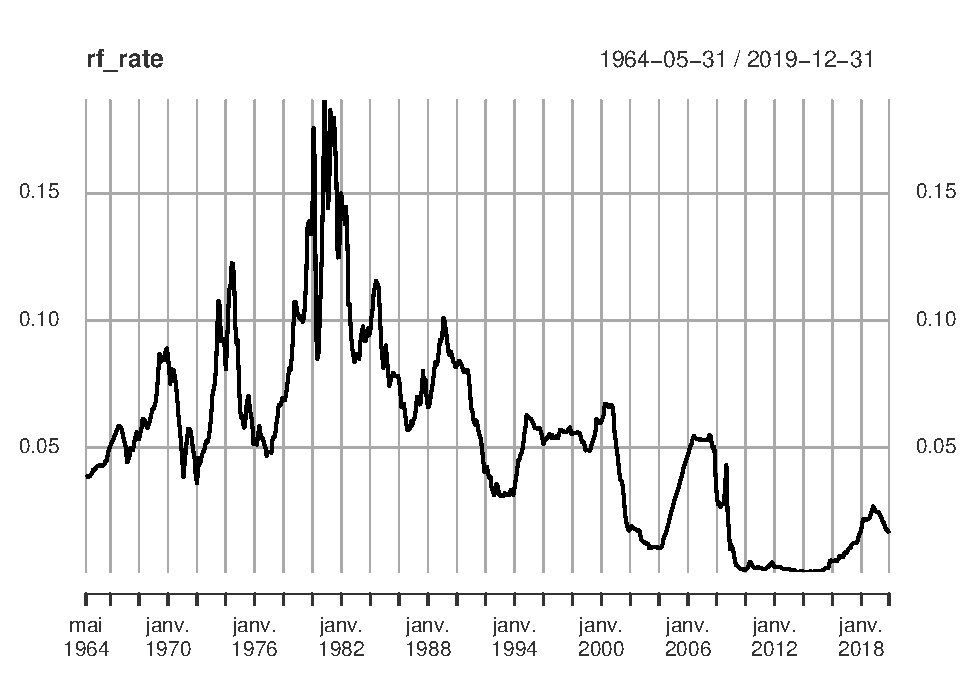
\includegraphics{TP-3_files/figure-latex/unnamed-chunk-6-1.pdf}

\begin{verbatim}
##                   AAPL        AMZN        MSFT            F          SPY
## 2008-06-30 -0.11290069 -0.10156825 -0.02860143 -0.292647079 -0.083575759
## 2008-07-31 -0.05070466  0.04104724 -0.06506746 -0.002079304 -0.008985578
## 2008-09-30 -0.32955848 -0.09961634 -0.02198624  0.165918802 -0.094173681
## 2008-10-31 -0.05340487 -0.21330401 -0.16335732 -0.578846139 -0.165186687
## 2008-12-31 -0.07899032  0.20093672 -0.03857552 -0.148698828  0.009796723
## 2009-03-31  0.17702424  0.13350827  0.13746188  0.314999474  0.083310627
##                    QQQ          XOM         MMM           HD           PG
## 2008-06-30 -0.09615030 -0.007097684 -0.10275897 -0.136855504 -0.079333799
## 2008-07-31  0.00642039 -0.087370994  0.01149577  0.017506396  0.083531745
## 2008-09-30 -0.15576296 -0.029371125 -0.04594999 -0.037367436 -0.001146315
## 2008-10-31 -0.15471594 -0.045583125 -0.05870276 -0.088837478 -0.067977481
## 2008-12-31  0.02277380 -0.003992837 -0.14029598  0.006785848 -0.039316221
## 2009-03-31  0.10316511  0.002945407  0.09370851  0.141905895 -0.022420454
##                      KO        Market           Rf
## 2008-06-30 -0.080159854 -0.0008065077 0.0023250000
## 2008-07-31 -0.009234303 -0.0268471854 0.0023250000
## 2008-09-30  0.030105361 -0.0910820596 0.0036000000
## 2008-10-31 -0.166793449 -0.2143686201 0.0019666667
## 2008-12-31 -0.034136711  0.0541143392 0.0008500000
## 2009-03-31  0.098898124  0.0883459620 0.0007416667
\end{verbatim}

\hypertarget{estimation-dun-moduxe8le-uxe0-un-facteur}{%
\section{Estimation d'un modèle à un
facteur}\label{estimation-dun-moduxe8le-uxe0-un-facteur}}

Choisir une période de 48 mois. A partir des exemples présentés en
cours, évaluer le modèle:

\[
R_i(t) - R_f(t) = \alpha + \beta (R_M(t) - R_f(t)) + \epsilon(t)
\]

en utilisant la fonction \texttt{lm}. Utilisez la fonction
\texttt{kable} de \texttt{knitr} pour produire une présentation soignée
des résultats.

\hypertarget{duxe9termination-du-portefeuille-actif}{%
\section{Détermination du portefeuille
actif}\label{duxe9termination-du-portefeuille-actif}}

On rappelle que le poids de chaque titre dans le portefeuille actif est
proportionnel au ratio \(\alpha_i/\sigma^2(\epsilon_i)\):

\[
w_i = \frac{\alpha_i/\sigma^2(\epsilon_i)}{\sum_i \alpha_i/\sigma^2(\epsilon_i)}
\]

Calculer les poids des actifs dans le portefeuille actif. Justifier
votre choix d'inclure ou d'exclure tel ou tel instrument.

Calculez les valeurs suivantes concernant le portefeuille actif:

\begin{description}
\item[$R_A$] Excess de rendement
\item[$\alpha_A$] alpha du portefeuille actif
\item[$\beta_A$]  beta du portefeuille actif
\item[$\sigma_A$] ecart-type du portefeuille actif
\end{description}

\hypertarget{duxe9termination-de-la-ponduxe9ration-entre-le-portefeuille-actif-et-le-portefeuille-de-marchuxe9.}{%
\section{Détermination de la pondération entre le portefeuille actif et
le portefeuille de
marché.}\label{duxe9termination-de-la-ponduxe9ration-entre-le-portefeuille-actif-et-le-portefeuille-de-marchuxe9.}}

On rappelle l'allocation de richesse au portefeuille actif:

\[
w_A = \frac{\alpha_A \sigma^2_M}{\alpha_A \sigma^2_M (1-\beta_A) + R_M \sigma^2_A}
\]

Avec:

\[
\begin{aligned}
R_A & = \alpha_A + \beta_A R_M \\
\sigma^2_A & = \beta^2_A \sigma^2_M + \sigma^2(\epsilon_A)
\end{aligned}
\]

Que penser de l'importance accordée au portefeuille actif?

\hypertarget{capital-allocation-line}{%
\section{Capital Allocation Line}\label{capital-allocation-line}}

Calculez l'espérance de rendement et le risque de quelques portefeuilles
situés sur la ``Capital Allocation Line'' qui joint l'actif sans risque
et le portefeuille risqué. Placez le portefeuille risqué, le
portefeuille actif et le portefeuille de marché sur un graphique
``excédent de rendement/risque,'' ci-dessous.

\begin{Shaded}
\begin{Highlighting}[]
\NormalTok{Assets }\OtherTok{\textless{}{-}} \FunctionTok{c}\NormalTok{(}\StringTok{"AAPL"}\NormalTok{, }\StringTok{"AMZN"}\NormalTok{, }\StringTok{"MSFT"}\NormalTok{, }\StringTok{"F"}\NormalTok{,  }\StringTok{"XOM"}\NormalTok{, }\StringTok{"MMM"}\NormalTok{,  }\StringTok{"HD"}\NormalTok{,   }\StringTok{"PG"}\NormalTok{,   }\StringTok{"KO"}\NormalTok{)}
\NormalTok{plot.data }\OtherTok{\textless{}{-}}\NormalTok{ monthly.ret}\FloatTok{.2}\NormalTok{[, }\FunctionTok{c}\NormalTok{(Assets, }\StringTok{"Rf"}\NormalTok{)]}
\ControlFlowTok{for}\NormalTok{(a }\ControlFlowTok{in}\NormalTok{ Assets) \{}
\NormalTok{  plot.data[, a] }\OtherTok{\textless{}{-}}\NormalTok{ plot.data[, a] }\SpecialCharTok{{-}}\NormalTok{ plot.data}\SpecialCharTok{$}\NormalTok{Rf}
\NormalTok{  \}}

\NormalTok{res }\OtherTok{\textless{}{-}} \FunctionTok{data.frame}\NormalTok{(}\AttributeTok{Mean=}\FunctionTok{apply}\NormalTok{(plot.data[, Assets],}\DecValTok{2}\NormalTok{,mean),}
                  \AttributeTok{Sd =} \FunctionTok{apply}\NormalTok{(plot.data[, Assets],}\DecValTok{2}\NormalTok{,sd))}
\FunctionTok{rownames}\NormalTok{(res) }\OtherTok{\textless{}{-}}\NormalTok{ Assets}
\end{Highlighting}
\end{Shaded}

\begin{Shaded}
\begin{Highlighting}[]
\FunctionTok{plot}\NormalTok{(Mean }\SpecialCharTok{\textasciitilde{}}\NormalTok{ Sd, }\AttributeTok{data=}\NormalTok{res, }\AttributeTok{xlim=}\FunctionTok{c}\NormalTok{(}\DecValTok{0}\NormalTok{, }\FloatTok{0.4}\NormalTok{), }\AttributeTok{ylim=}\FunctionTok{c}\NormalTok{(}\DecValTok{0}\NormalTok{, .}\DecValTok{05}\NormalTok{), }\AttributeTok{xlab=}\FunctionTok{expression}\NormalTok{(sigma),}
     \AttributeTok{ylab=}\StringTok{"Excess Return"}\NormalTok{, }\AttributeTok{cex=}\NormalTok{.}\DecValTok{5}\NormalTok{, }\AttributeTok{bty=}\StringTok{"n"}\NormalTok{, }\AttributeTok{cex.lab=}\DecValTok{1}\NormalTok{)}
\FunctionTok{with}\NormalTok{(res, }\FunctionTok{text}\NormalTok{(Mean }\SpecialCharTok{\textasciitilde{}}\NormalTok{ Sd, }\AttributeTok{labels=}\FunctionTok{row.names}\NormalTok{(res), }\AttributeTok{pos=}\DecValTok{4}\NormalTok{, }\AttributeTok{cex=}\FloatTok{0.5}\NormalTok{, }\AttributeTok{col=}\StringTok{"blue"}\NormalTok{))}
\end{Highlighting}
\end{Shaded}

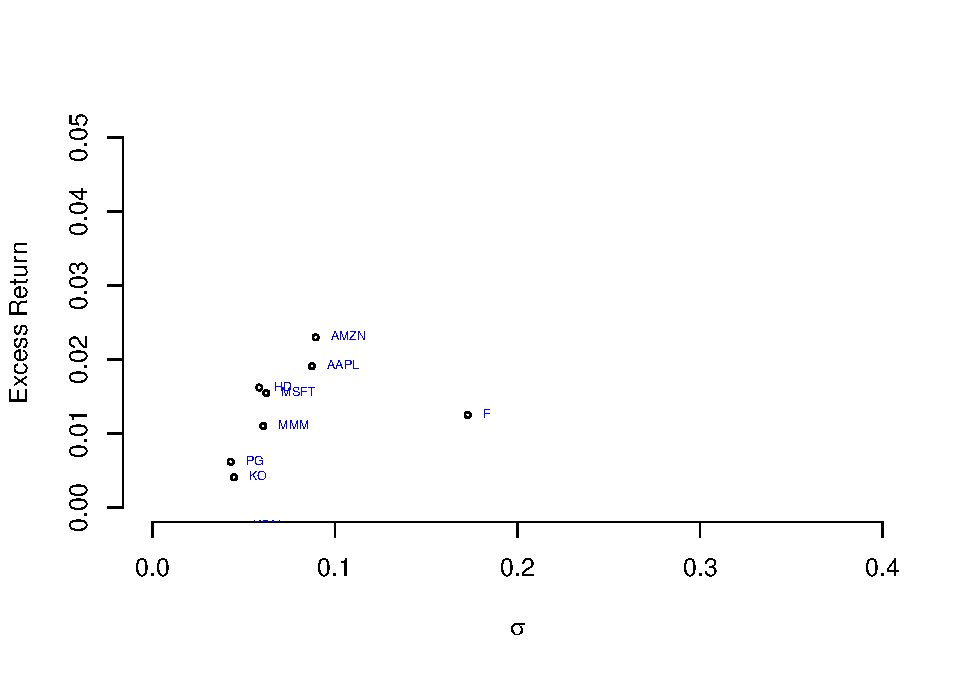
\includegraphics{TP-3_files/figure-latex/unnamed-chunk-9-1.pdf}

\end{document}
